\subsection{Expression of Human and Bovine IFITs} \label{Expression of Human and Bovine IFITs}
\subsubsection{Validation Antibodies} \label{Validation Antibodies}
Overexpressed human IFITs \newline
figures

\begin{figure}
    \centering
    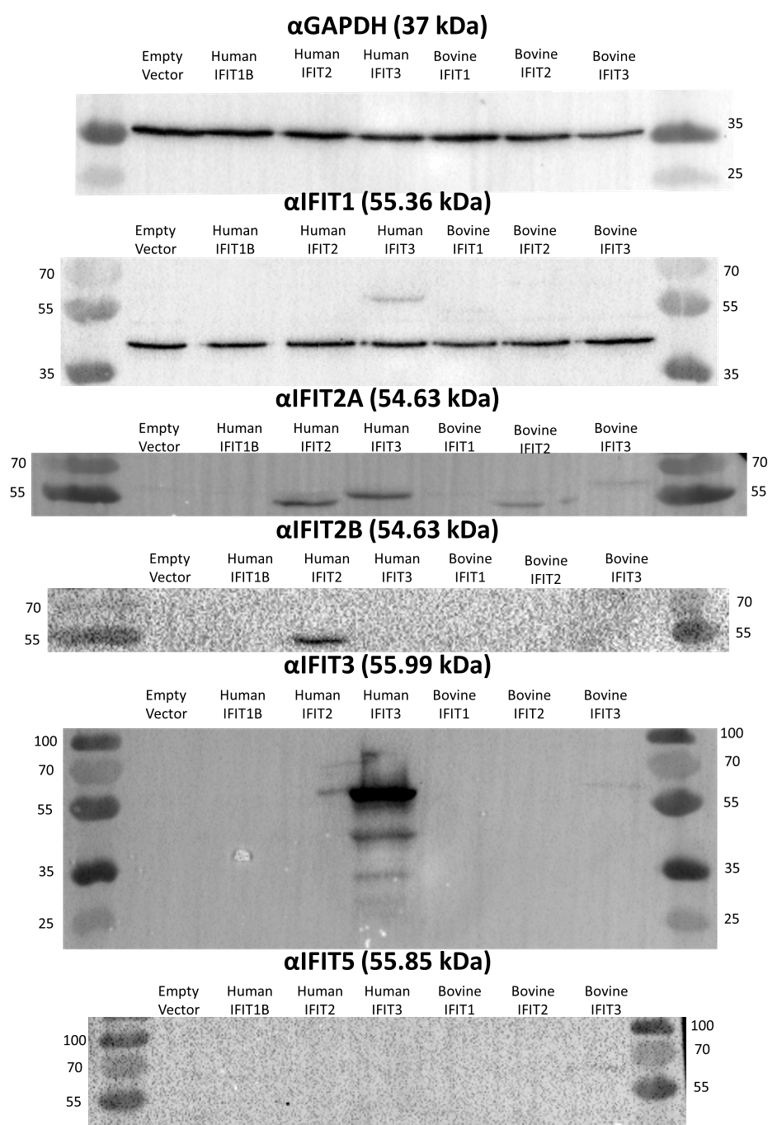
\includegraphics[width=0.5\linewidth]{06. Chapter 1/Figs/02. Expression/01. atb-validation.png}
    \caption[Human IFIT antibody validation.]{\textbf{Human IFIT antibody validation.} test test test test test test test test test test test.}
    \label{Human IFIT antibody validation.} 
\end{figure}

\subsubsection{Western Blots of Treatment and Infection} \label{Western Blots of Treatment and Infection}
Western of time course of treatment with IFN etc. (GAPDH, IFITs) \newline
Western of infection time course (N, P, GAPDH, IFITs) \newline
A549, BEAS2B

\begin{figure}
    \centering
    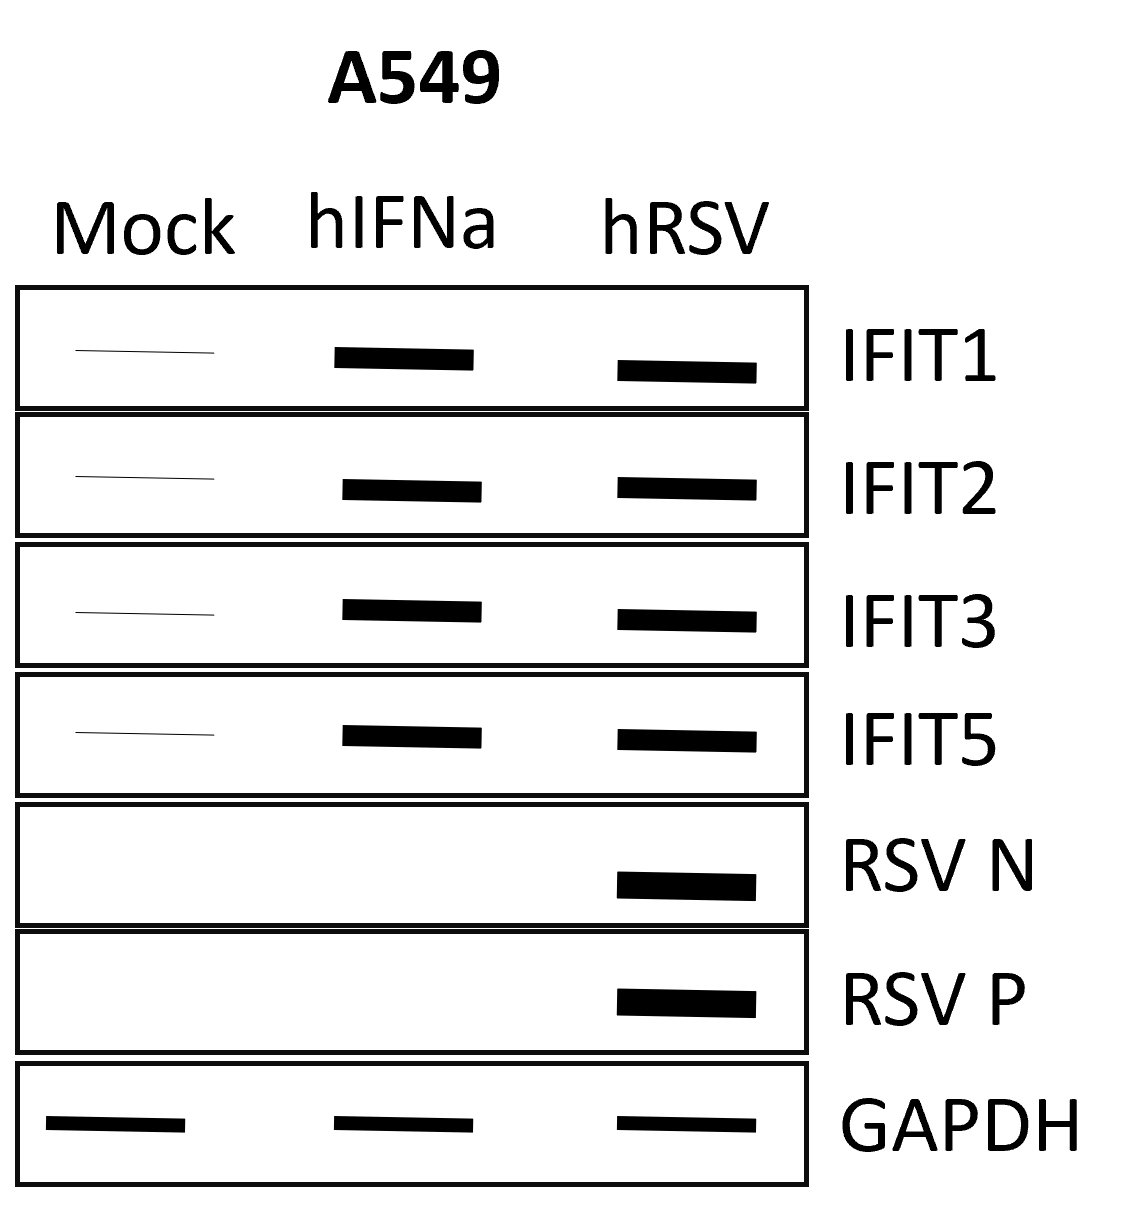
\includegraphics[width=0.5\linewidth]{06. Chapter 1/Figs/02. Expression/02. A549 WB.png}
    \caption[A549 Western Blot.]{\textbf{A549 Western Blot.} test test test test test test test test test test test.}
    \label{A549 Western Blot.}
\end{figure}

\begin{figure}
    \centering
    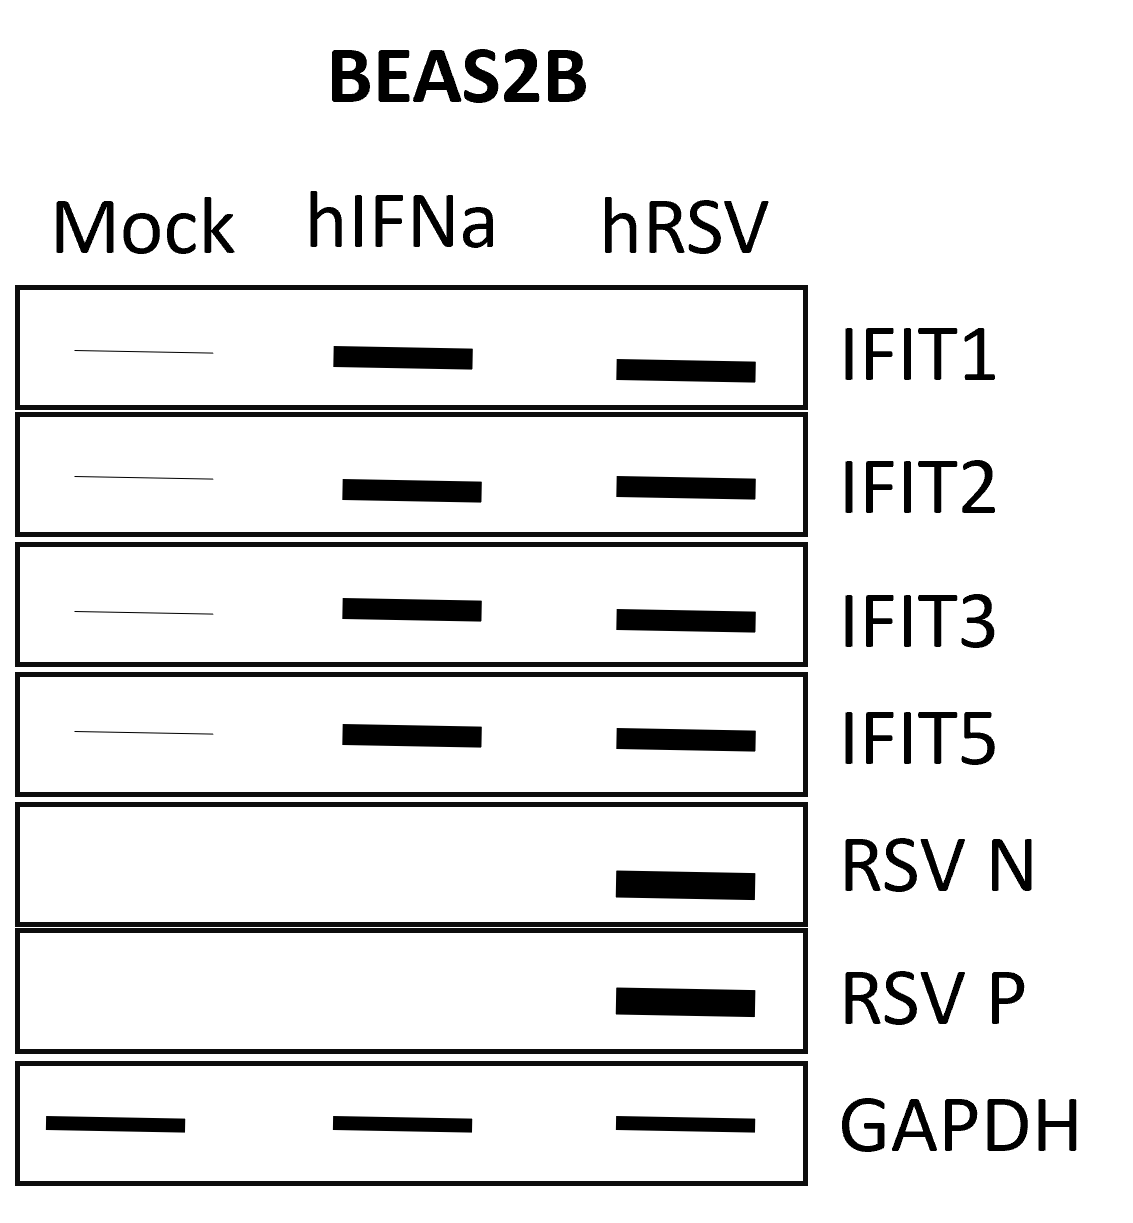
\includegraphics[width=0.5\linewidth]{06. Chapter 1/Figs/02. Expression/03. beas2b wb.png}
    \caption[BEAS-2B Western Blot.]{\textbf{BEAS-2B Western Blot.} test test test test test test test test test test test.}
    \label{BEAS-2B Western Blot.}
\end{figure}

\subsubsection{Validation by Comparing to the Proteomic Dataset} \label{Validation by Comparing to the Proteomic Dataset}
Who, what and why it was done  \newline
Cite the bioArchive paper \cite{Jobe2023ViralCondensates}

\begin{figure}
    \centering
    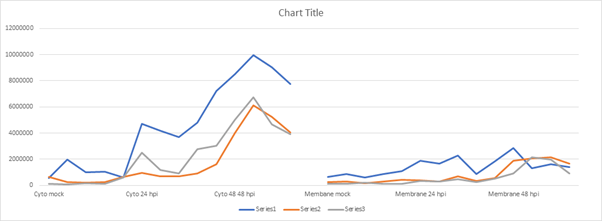
\includegraphics[width=1\linewidth]{06. Chapter 1/Figs/02. Expression/04. proteomics.png}
    \caption[Human IFIT proteins detected per fraction.]{\textbf{Human IFIT proteins detected per fraction.} test test test test test test test test test test test.}
    \label{Human IFIT proteins detected per fraction.}
\end{figure}

Describe data: \newline
asdasdasd \newline
Proteomics dataset from Dalan’s lab looking at differential enrichment of proteins between membrane and cytosolic fractures. It confirms that in A549 (I think) IFITs 1 (series 1), 2 (series 2) and 3 (series 3) are induced in the cytosolic fraction at protein level 







\subsubsection{Western Blots of Treatment and Infection} \label{Western Blots of Treatment and Infection}
Western of time course of treatment with IFN etc. (GAPDH, IFITs) \newline
Western of infection time course (N, P, GAPDH, IFITs) \newline
MDBK, BT

\begin{figure}
    \centering
    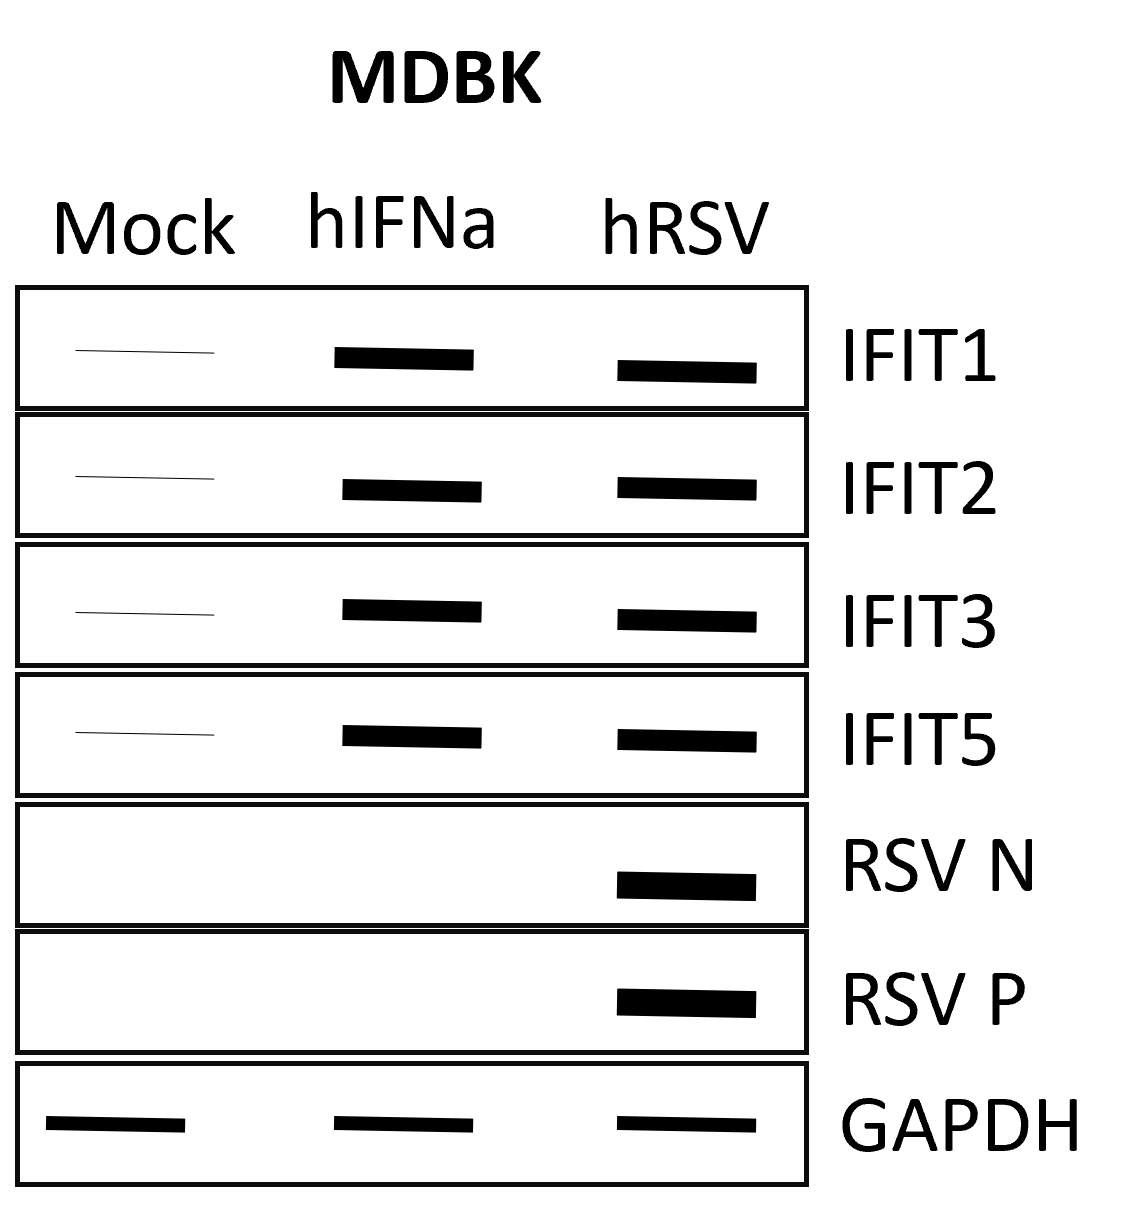
\includegraphics[width=0.5\linewidth]{07. Chapter 2/Figs/03. Expression/02. mdbk wb.png}
    \caption[MDBK Western Blot.]{\textbf{MDBK Western Blot.} test test test test test test test test test test test.}
    \label{MDBK Western Blot.}
\end{figure}

\begin{figure}
    \centering
    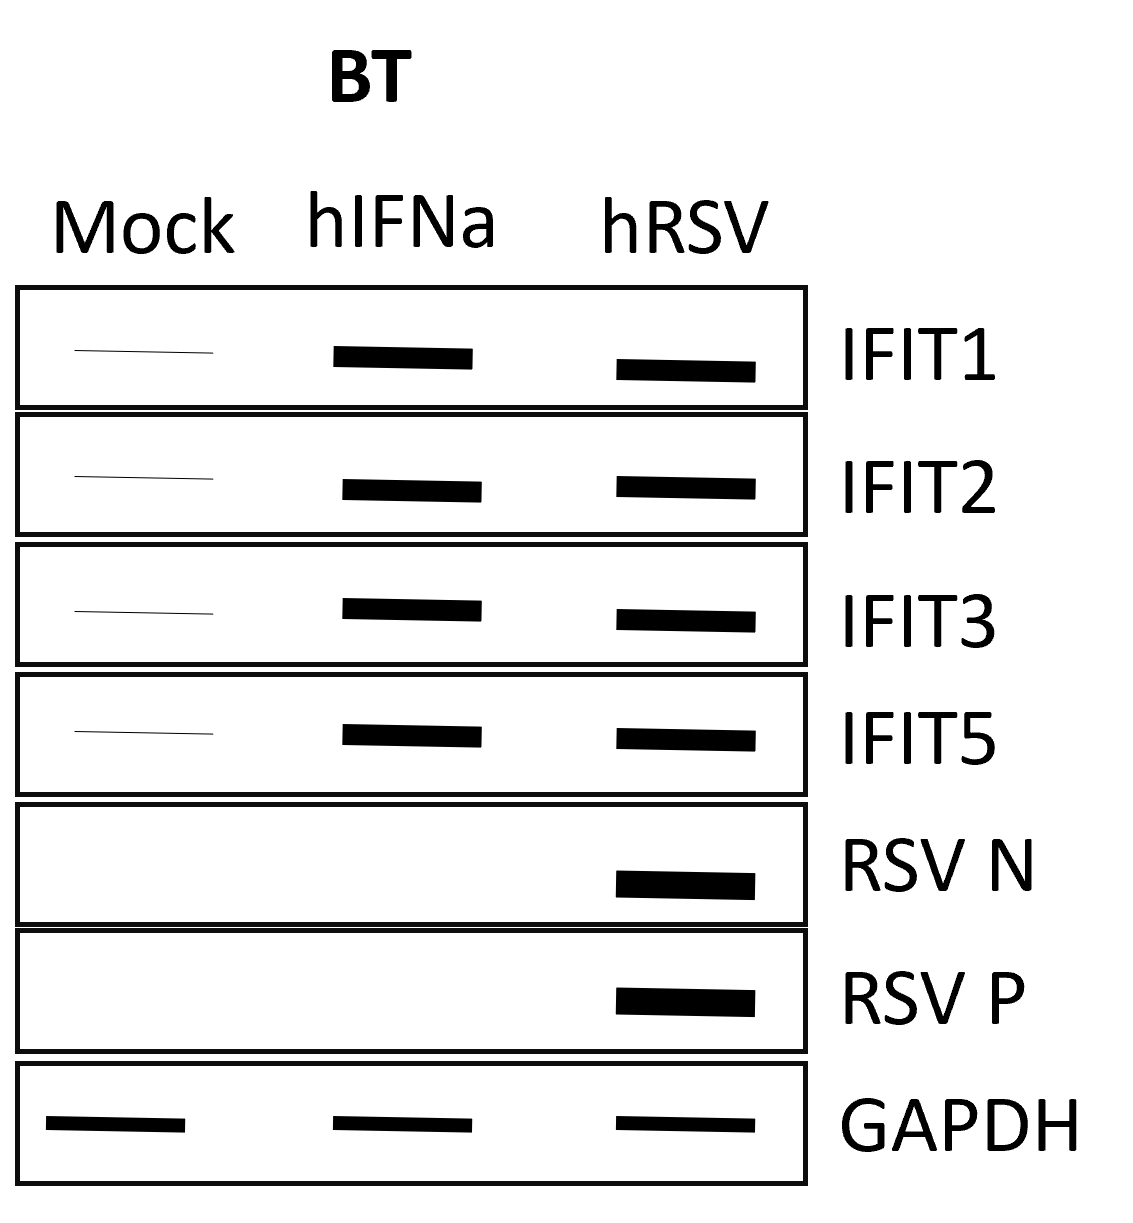
\includegraphics[width=0.5\linewidth]{07. Chapter 2/Figs/03. Expression/03. bt wb.png}
    \caption[BT Western Blot.]{\textbf{BT Western Blot.} test test test test test test test test test test test.}
    \label{BT Western Blot.}
\end{figure}
